\documentclass{article}
\usepackage[margin=1in]{geometry}
%\documentclass[]{aiaa-tc}% insert '[draft]' option to show overfull boxes
\usepackage[utf8]{inputenc}
\usepackage{amsmath}
\usepackage{float}
\usepackage{graphicx} % needed for figures
\usepackage{tabularx}
\usepackage[mathscr]{euscript}
\usepackage{graphicx}
\graphicspath{ {figures/} }
\title{ECEN 773 Semester Project}
\author{Dustan Kraus}
\date{April 2017}

\begin{document}

\maketitle

\section{Introduction}
For my thesis, I am researching multi-arm manipulation. My initial approach with this is to implement an object level controller. Using a dynamic model of the object to be manipulated, I will predict the forces and torques required to cause desired object motion. Eventually, I will need to design an outer loop controller for the robotic manipulators to apply these forces and torques. However, first, I need to work on the inner loop (the object model and control). Prior to this project, I hadn't done any work on this specific aspect of my project. So, I determined that it would help both my research progress and my understanding of the control theory I have learned in this class to derive a dynamic model for an object being manipulated, linearize that model, and then implement the control principles I've learned in this class on the linearized and non-linear model.

\section{Object Model Derivation and Linearization}
Any object of mass $m$ has an inertia matrix defined by Eqn.~\ref{eq:I}. 
\begin{equation}\label{eq:I}
%\begin{aligned}
I=
  \begin{bmatrix}
    I_{xx} & -I_{xy} & -I_{xz} \\
    -I_{xy} & I_{yy} & -I_{yz} \\
    -I_{xz} & -I_{yz} & I_{zz}
  \end{bmatrix}
%\end{aligned}
\end{equation}
There are n locations on the object where forces and torques are applied in the x, y, and z directions (by n manipulators). The forces are applied at dx, dy, and dz from the center of mass of the object. Given the inertia matrix, the forces and torques applied, and the application locations of the forces and torques, I derived the dynamic equations shown below. Since the derivation of the dynamics is outside of the scope of this class, I won't go into details about how I derived these equations. I will say that the derivation was not trivial and took a lot of time, but the focus of this paper is the linear control of this dynamical system rather than its derivation. The twelve 1st-order equations are shown in Eqs.~\ref{eq:xdot} - ~\ref{eq:Torque}. Note that I used $c_{\theta}$ to represent $cos(\theta)$ so that the equations would fit. The variables used are defined in Table~\ref{tab:variable_definition}.
\noindent
\begin{table}[H]
\centering
\begin{tabularx}{0.99\textwidth}{|X|X|}%{ |m{4cm}|m{3cm}|}
%\begin{tabu} to 0.99\textwidth { | X[lm] | X[rm] | }
 \hline
 $\omega_x$ & \multicolumn{1}{|r|}{Angular velocity about body fixed x-axis} \\%[3em]
 \hline
 $\omega_y$ & \multicolumn{1}{|r|}{Angular velocity about body fixed y-axis} \\%[3em]
 \hline
 $\omega_z$ & \multicolumn{1}{|r|}{Angular velocity about body fixed z-axis} \\%[3em]
 \hline
 $\psi$  & \multicolumn{1}{|r|}{Euler angle yaw about inertial z-axis} \\%[1em]
 \hline
 $\theta$  & \multicolumn{1}{|r|}{Euler angle pitch about intermediate y-axis} \\%[1em]
 \hline
 $\phi$  & \multicolumn{1}{|r|}{Euler angle roll about body fixed x-axis} \\%[1em]
 \hline  
 $p_x$  & \multicolumn{1}{|r|}{Object center of mass x position relative to and in terms of inertial x-axis} \\%[1em]
 \hline 
 $p_y$  & \multicolumn{1}{|r|}{Object center of mass y position relative to and in terms of inertial y-axis} \\%[1em]
 \hline 
 $p_z$  & \multicolumn{1}{|r|}{Object center of mass z position relative to and in terms of inertial y-axis} \\%[1em]
 \hline
 $v_x$  & \multicolumn{1}{|r|}{Object center of mass x velocity relative to inertial frame and in terms of body fixed x-axis} \\%[1em]
 \hline 
 $v_y$  & \multicolumn{1}{|r|}{Object center of mass y velocity relative to inertial frame and in terms of body fixed y-axis} \\%[1em]
 \hline
 $v_z$  & \multicolumn{1}{|r|}{Object center of mass z velocity relative to inertial frame and in terms of body fixed z-axis} \\%[1em]
 \hline  
\end{tabularx}
\caption{This table contains definitions of the variables used in the dynamic equations (Eqs.~\ref{eq:xdot} and \ref{eq:Torque}).}
\label{tab:variable_definition}
\end{table}

\begin{equation}\label{eq:xdot}
\dot{x}=
\begin{bmatrix}
\dot{\omega_x} \\
\dot{\omega_y} \\
\dot{\omega_z} \\
\dot{\psi} \\
\dot{\theta} \\
\dot{\phi} \\
\dot{p_x} \\
\dot{p_y} \\
\dot{p_z} \\
\dot{v_x} \\
\dot{v_y} \\
\dot{v_z} \\
\end{bmatrix}=
\begin{bmatrix}
  \begin{bmatrix}
    I_{xx} & -I_{xy} & -I_{xz} \\
    -I_{xy} & I_{yy} & -I_{yz} \\
    -I_{xz} & -I_{yz} & I_{zz}
  \end{bmatrix}^{-1}  \begin{bmatrix}
  -I_{xy} \omega_x \omega_z + I_{xz} \omega_x \omega_y + (I_{yy} - I_{zz}) \omega_y \omega_z + I_{yz} (\omega_y^2 - \omega_z^2) + T_x \\
  -I_{yz} \omega_x \omega_y + I_{xy} \omega_y \omega_z + (I_{zz} - I_{xx}) \omega_x \omega_z + I_{xz} (\omega_z^2 - \omega_x^2) + T_y \\
  -I_{xz} \omega_y \omega_z + I_{yz} \omega_x \omega_z + (I_{xx} - I_{yy}) \omega_x \omega_y + I_{xy} (\omega_x^2 - \omega_y^2) + T_z
  \end{bmatrix} \\
\dfrac{1}{c_{\theta}}(\omega_y s_{\phi} + \omega_z c_{\phi}) \\
\omega_y c_{\phi} - \omega_z s_{\phi} \\
\dfrac{1}{c_{\theta}} (\omega_y s_{\theta} s_{\phi} + \omega_z s_{\theta} c_{\phi}) + \omega_x \\
v_x c_{\psi} c_{\theta} - v_y(c_{\phi}s_{\psi} - c_{\psi}s_{\phi}s_{\theta}) + v_z(s_{\psi}s_{\phi} + c_{\phi}c_{\psi}s_{\theta})\\
v_x c_{\theta} s_{\psi} + v_y(c_{phi}c_{\psi} + s_{\phi}s_{\psi}s_{\theta}) - v_z(c_{\psi}s_{\phi} - c_{\phi}s_{\psi}s_{\theta}) \\
-v_x s_{\theta} + v_y c_{\theta}s_{\phi} + v_z c_{\phi} c_{\theta} \\
\dfrac{1}{m} (\sum_{i=1}^{n} F_{xi}) + g s_{\theta} - v_z \omega_y + v_y \omega_z \\
\dfrac{1}{m} (\sum_{i=1}^{n} F_{yi}) - g c_{\theta} s_{\phi} + v_z \omega_x - v_x \omega_z \\
\dfrac{1}{m} (\sum_{i=1}^{n} F_{zi}) - g c_{\theta} c_{\phi} - v_y \omega_x + v_x \omega_y
  \end{bmatrix}
\end{equation}

\begin{equation}\label{eq:Torque}
\begin{bmatrix}
T_x \\
T_y \\
T_z
\end{bmatrix}=
\begin{bmatrix}
\sum_{i=1}^{n} T_{xi} + F_{zi} dy_i - F_{yi} dz_i \\
\sum_{i=1}^{n} T_{yi} + F_{xi} dz_i - F_{zi} dx_i \\
\sum_{i=1}^{n} T_{zi} + F_{xi} dy_i - F_{yi} dx_i
\end{bmatrix}
\end{equation}

The forces and torques appear in 6 of the 12 dynamic equations. So, in order to be able to simply solve for the equilibrium inputs, I let there only be one location where forces and torques are applied. This resulted in 6 equations and 6 unknowns (force and torque in x, y, and z at the given location) that I could solve for the equilibrium forces and torques. Using this system, I set all the state variable derivatives ($\dot{x}$) equal to zero and found the equilibrium forces and torques shown in Eq.~\ref{eq:equilibrium}. 

\begin{equation}\label{eq:equilibrium}
u_{eq}=
\begin{bmatrix}
T_{x,eq} \\
T_{y,eq} \\
T_{z,eq} \\
F_{x,eq} \\
F_{y,eq} \\
F_{z,eq}
\end{bmatrix}=
\begin{bmatrix}
1 & 0 & 0 & 0 & -dz & dy \\
0 & 1 & 0 & dz & 0 & -dx \\
0 & 0 & 1 & -dy & dx & 0 \\
0 & 0 & 0 & \dfrac{1}{m} & 0 & 0 \\
0 & 0 & 0 & 0 & \dfrac{1}{m} & 0  \\
0 & 0 & 0 & 0 & 0 & \dfrac{1}{m} 
\end{bmatrix}^{-1}
\begin{bmatrix}
0 \\
0 \\
0 \\
0 \\
0 \\
g \\
\end{bmatrix}
\end{equation}

I chose my object to be a rectangular prism, chose values for system parameters, and then linearized the equations about 0 for all the states where A, B, C, and D are shown below in Eqs.~\ref{eq:A} - \ref{eq:D}.

\begin{equation}\label{eq:A}
A=
  \begin{bmatrix}
    \frac{\partial f_1}{\partial x_1} & \frac{\partial f_1}{\partial x_2} & \dots  & \frac{\partial f_1}{\partial x_{12}} \\ \\
    \frac{\partial f_2}{\partial x_1} & \frac{\partial f_2}{\partial x_2} & \dots  & \frac{\partial f_2}{\partial x_{12}} \\
    \vdots &  & \ddots  &  \\
    \frac{\partial f_{12}}{\partial x_1} & \frac{\partial f_{12}}{\partial x_2} & \dots  & \frac{\partial f_{12}}{\partial x_{12}}
  \end{bmatrix}=
  \setcounter{MaxMatrixCols}{20}
  \begin{bmatrix}
  0 & 0 & 0 & 0 & 0 & 0 & 0 & 0 & 0 & 0 & 0 & 0 \\ 
  0 & 0 & 0 & 0 & 0 & 0 & 0 & 0 & 0 & 0 & 0 & 0 \\ 
  0 & 0 & 0 & 0 & 0 & 0 & 0 & 0 & 0 & 0 & 0 & 0 \\
  0 & 0 & 1 & 0 & 0 & 0 & 0 & 0 & 0 & 0 & 0 & 0 \\ 
  0 & 1 & 0 & 0 & 0 & 0 & 0 & 0 & 0 & 0 & 0 & 0 \\ 
  1 & 0 & 0 & 0 & 0 & 0 & 0 & 0 & 0 & 0 & 0 & 0 \\ 
  0 & 0 & 0 & 0 & 0 & 0 & 0 & 0 & 0 & 1 & 0 & 0 \\ 
  0 & 0 & 0 & 0 & 0 & 0 & 0 & 0 & 0 & 0 & 1 & 0 \\ 
  0 & 0 & 0 & 0 & 0 & 0 & 0 & 0 & 0 & 0 & 0 & 1 \\ 
  0 & 0 & 0 & 0 & g & 0 & 0 & 0 & 0 & 0 & 0 & 0 \\ 
  0 & 0 & 0 & 0 & 0 & -g & 0 & 0 & 0 & 0 & 0 & 0 \\ 
  0 & 0 & 0 & 0 & 0 & 0 & 0 & 0 & 0 & 0 & 0 & 0 \\  
  \end{bmatrix}
\end{equation}
\begin{equation}\label{eq:B}
B=
  \begin{bmatrix}
    \frac{\partial f_1}{\partial u_1} & \frac{\partial f_1}{\partial u_2} & \dots  & \frac{\partial f_1}{\partial u_6} \\ \\
    \frac{\partial f_2}{\partial u_1} & \frac{\partial f_2}{\partial u_2} & \dots  & \frac{\partial f_2}{\partial u_6} \\
    \vdots &  & \ddots  &  \\
    \frac{\partial f_{12}}{\partial u_1} & \frac{\partial f_{12}}{\partial u_2} & \dots  & \frac{\partial f_{12}}{\partial u_6}
  \end{bmatrix}=
  \setcounter{MaxMatrixCols}{20}
  \begin{bmatrix}
  \dfrac{16}{17} & 0 & 0 & 0 & \dfrac{-8}{85} & \dfrac{32}{85} \\
  0 & \dfrac{16}{5} & 0 & \dfrac{8}{25} & 0 & \dfrac{-16}{25} \\
  0 & 0 & \dfrac{4}{5} & \dfrac{-8}{25} & \dfrac{4}{25} & 0 \\
  0 & 0 & 0 & 0 & 0 & 0 \\
  0 & 0 & 0 & 0 & 0 & 0 \\
  0 & 0 & 0 & 0 & 0 & 0 \\
  0 & 0 & 0 & 0 & 0 & 0 \\
  0 & 0 & 0 & 0 & 0 & 0 \\
  0 & 0 & 0 & 0 & 0 & 0 \\
  0 & 0 & 0 & \dfrac{1}{12} & 0 & 0 \\
  0 & 0 & 0 & 0 & \dfrac{1}{12} & 0 \\
  0 & 0 & 0 & 0 & 0 & \dfrac{1}{12} 
  \end{bmatrix}
\end{equation}
\begin{equation}\label{eq:C}
C=
  \begin{bmatrix}
  0 & 0 & 0 & 1 & 0 & 0 & 0 & 0 & 0 & 0 & 0 & 0 \\ 
  0 & 0 & 0 & 0 & 1 & 0 & 0 & 0 & 0 & 0 & 0 & 0 \\ 
  0 & 0 & 0 & 0 & 0 & 1 & 0 & 0 & 0 & 0 & 0 & 0 \\
  0 & 0 & 0 & 0 & 0 & 0 & 1 & 0 & 0 & 0 & 0 & 0 \\ 
  0 & 0 & 0 & 0 & 0 & 0 & 0 & 1 & 0 & 0 & 0 & 0 \\ 
  0 & 0 & 0 & 0 & 0 & 0 & 0 & 0 & 1 & 0 & 0 & 0 
  \end{bmatrix}
\end{equation}  
\begin{equation}\label{eq:D}
D=
  \begin{bmatrix}
  0 & 0 & 0 & 0 & 0 & 0 \\
  0 & 0 & 0 & 0 & 0 & 0 \\
  0 & 0 & 0 & 0 & 0 & 0 \\
  0 & 0 & 0 & 0 & 0 & 0 \\
  0 & 0 & 0 & 0 & 0 & 0 \\
  0 & 0 & 0 & 0 & 0 & 0 
  \end{bmatrix}
\end{equation}

\section{LQR/LQG Control}
After finding the linearized equations, I wanted to ensure that the system was controllable and observable, so I computed the controllability and observability matrices as shown in Eqs.~\ref{eq:observability}-\ref{eq:controllability}. I found that the rank of each of these matrices was 12 which is equal to the number of states I was using, so the system is both observable and controllable.

\begin{equation}\label{eq:observability}
\mathscr{O}=
\begin{bmatrix}
C \\
CA \\
CA^2 \\
\vdots \\
CA^{11}
\end{bmatrix}
\end{equation}

\begin{equation}\label{eq:controllability}
\mathscr{C}=
\begin{bmatrix}
B & AB & A^2B & \dots & A^{11}B
\end{bmatrix}
\end{equation}

After determining that the linear system was controllable and observable, I preceded with the LQR design by selecting Q and R matrices. I started by selecting entries of the Q and R matrices using Bryson's rule, and then slightly adjusted the values to get the response I wanted. The Q and R matrices I ended up using are shown in Eqs.~\ref{eq:Q}-\ref{eq:R}.

\begin{equation}\label{eq:Q}
Q=
  \begin{bmatrix}
  10 & 0 & 0 & 0 & 0 & 0 & 0 & 0 & 0 & 0 & 0 & 0 \\
  0 & 10 & 0 & 0 & 0 & 0 & 0 & 0 & 0 & 0 & 0 & 0 \\
  0 & 0 & 10 & 0 & 0 & 0 & 0 & 0 & 0 & 0 & 0 & 0 \\
  0 & 0 & 0 & 100 & 0 & 0 & 0 & 0 & 0 & 0 & 0 & 0 \\
  0 & 0 & 0 & 0 & 100 & 0 & 0 & 0 & 0 & 0 & 0 & 0 \\
  0 & 0 & 0 & 0 & 0 & 100 & 0 & 0 & 0 & 0 & 0 & 0 \\
  0 & 0 & 0 & 0 & 0 & 0 & 100 & 0 & 0 & 0 & 0 & 0 \\
  0 & 0 & 0 & 0 & 0 & 0 & 0 & 100 & 0 & 0 & 0 & 0 \\
  0 & 0 & 0 & 0 & 0 & 0 & 0 & 0 & 100 & 0 & 0 & 0 \\
  0 & 0 & 0 & 0 & 0 & 0 & 0 & 0 & 0 & 10 & 0 & 0 \\
  0 & 0 & 0 & 0 & 0 & 0 & 0 & 0 & 0 & 0 & 10 & 0 \\
  0 & 0 & 0 & 0 & 0 & 0 & 0 & 0 & 0 & 0 & 0 & 10 \\
  \end{bmatrix}
\end{equation}
\begin{equation}\label{eq:R}
R=
  \begin{bmatrix}
  0.1 & 0 & 0 & 0 & 0 & 0 \\
  0 & 0.1 & 0 & 0 & 0 & 0 \\
  0 & 0 & 0.1 & 0 & 0 & 0 \\
  0 & 0 & 0 & 0.1 & 0 & 0 \\
  0 & 0 & 0 & 0 & 0.1 & 0 \\
  0 & 0 & 0 & 0 & 0 & 0.1 
  \end{bmatrix}
\end{equation}

I then used MATLAB's lqr command to obtain the K gain matrix for optimal control. I then simulated the system using the full non-linear dynamic model shown in Eq.~\ref{eq:xdot} with state feedback $u = -Kx + u_{eq}$. I found that as I decreased the values in the R matrix, I was able to get much quicker responses with less overshoot, but the control inputs were much higher (see Figures~\ref{fig:R_0.1}-\ref{fig:R_0.001}).

\begin{figure}[H]
    \centering
        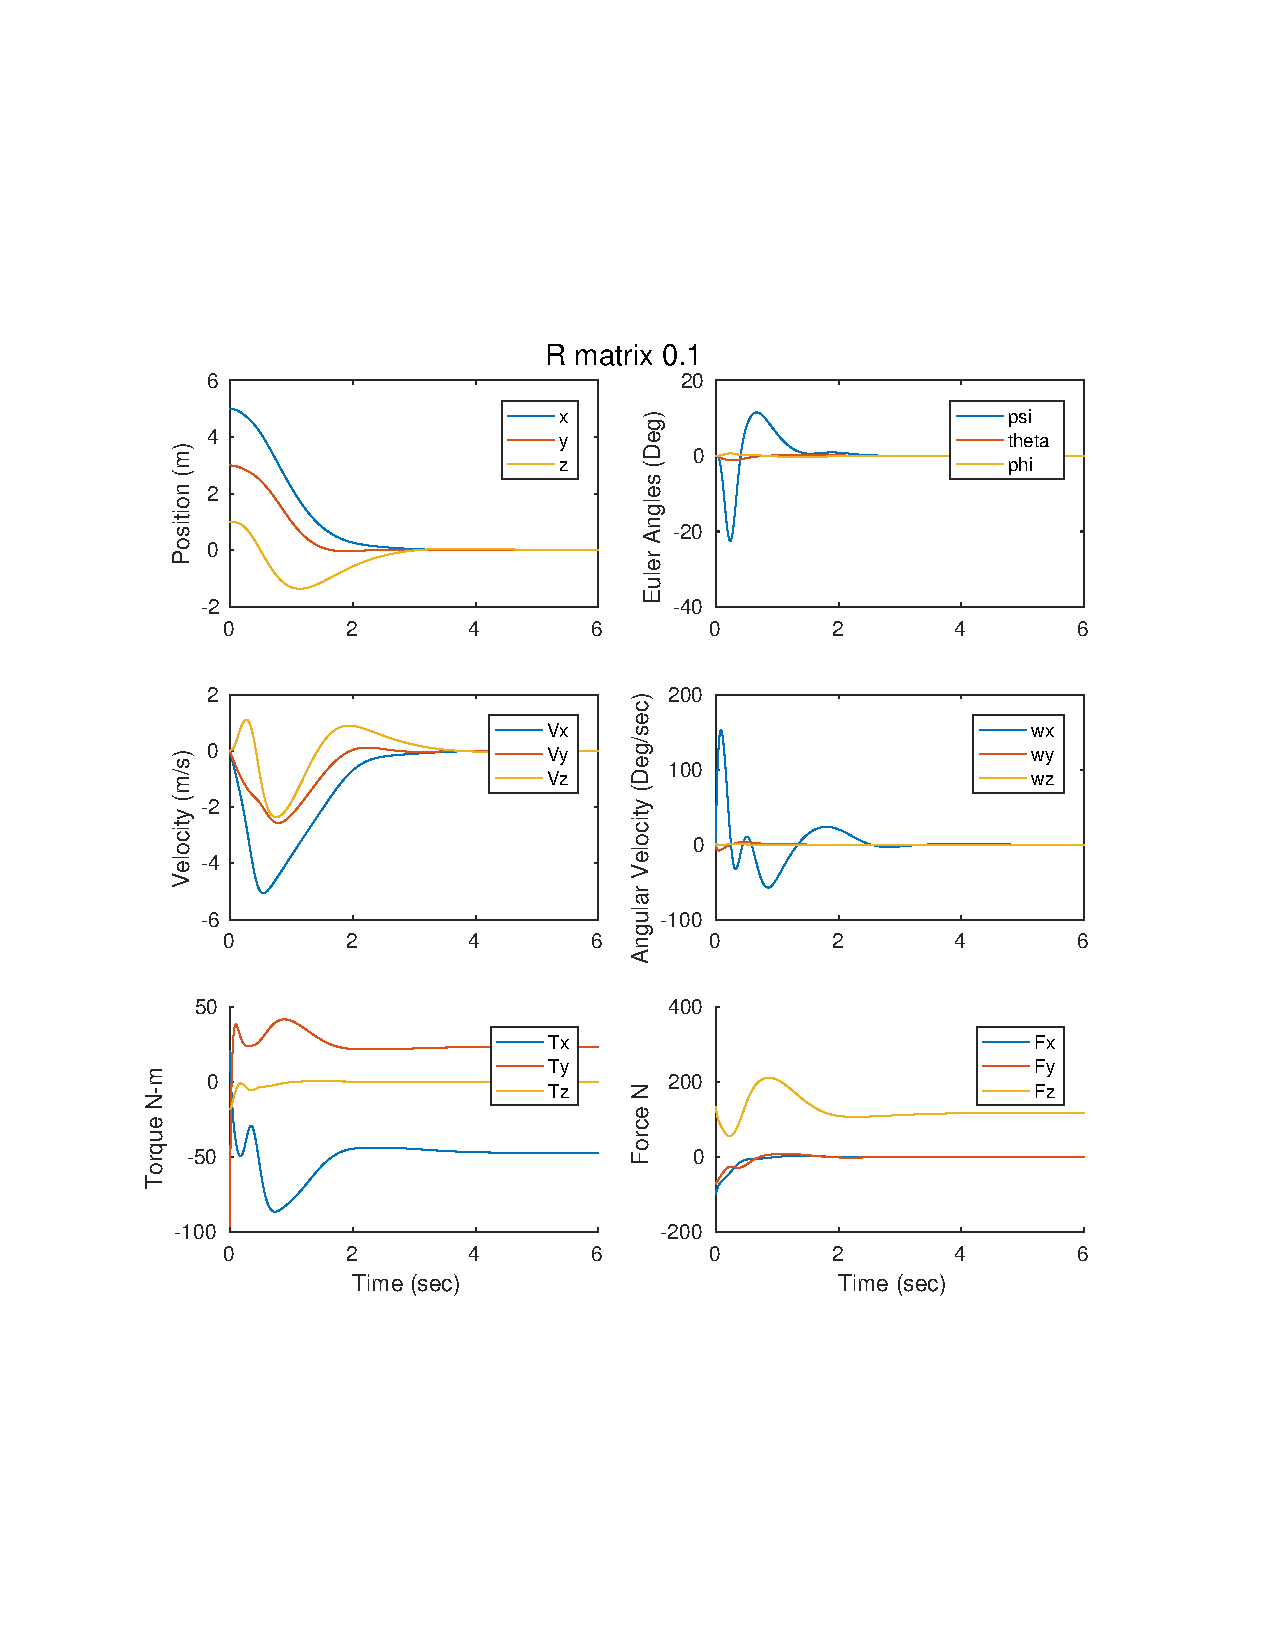
\includegraphics[clip, trim=2cm 6cm 3cm 5cm, width=0.69\textwidth]{R_0_1_plot.pdf}
    \caption{This figure contains the simulated response with R matrix value of 0.1 on the diagonal.}
    \label{fig:R_0.1}
\end{figure}

\begin{figure}[H]
\centering
  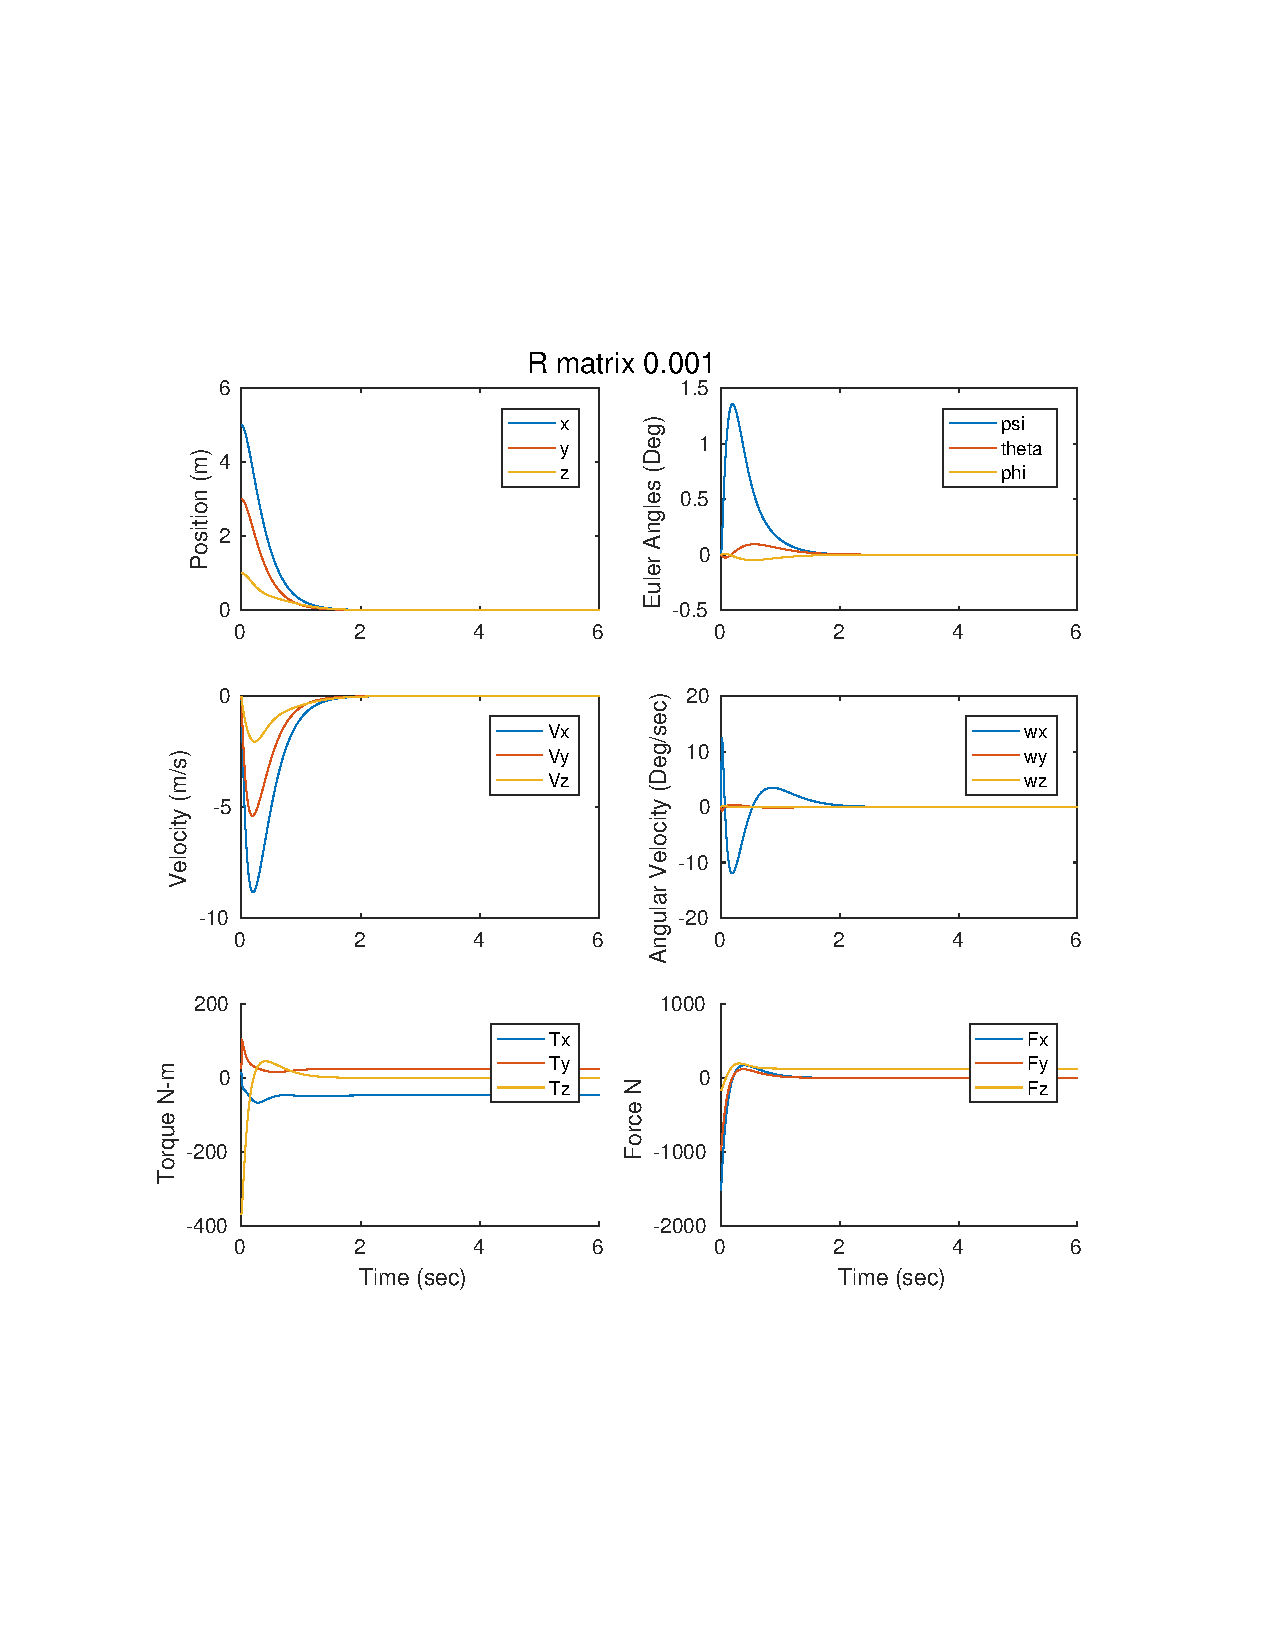
\includegraphics[clip, trim=2cm 6cm 3cm 5cm, width=0.69\textwidth]{R_0_001_plot}
  \caption{This figure contains the simulated response with R matrix value of 0.001 on the diagonal.}
  \label{fig:R_0.001}
\end{figure}

This was all assuming full state feedback; however, in the real system, I will be able to measure $\psi, \theta, \phi, p_x, p_y,$ and $p_z$ as shown by the C matrix in Eq.~\ref{eq:C}. I will measure these using an HTC vive tracker which I will place on the object. So, I made a state observer by solving the controllability algabraic ricatti equation using matlab's 'care' function where I passed in $A^T, C^T,$ and $Q$. I then set my observer gain matrix $L = S C^T N^{-1}$ where N is a gain matrix I also set. Using this gain matrix (L), I was able to estimate x as $\hat{x}$ by setting $\dot{\hat{x}} = (A-LC)\hat{x} + Bu + LCx$. In this case though, for the x multiplied by LC, I used the actual states for $\psi, \theta, \phi, p_x, p_y,$ and $p_z$ since they are measured, and the estimated states for the others. By doing this I was able to again simulate the system, but with the estimated states rather than the true states and got the response shown below in Figure~\ref{fig:est_states}. The response is a bit worse, but only because it takes a little bit for the state estimates to become accurate.

\begin{figure}[H]
    \centering
        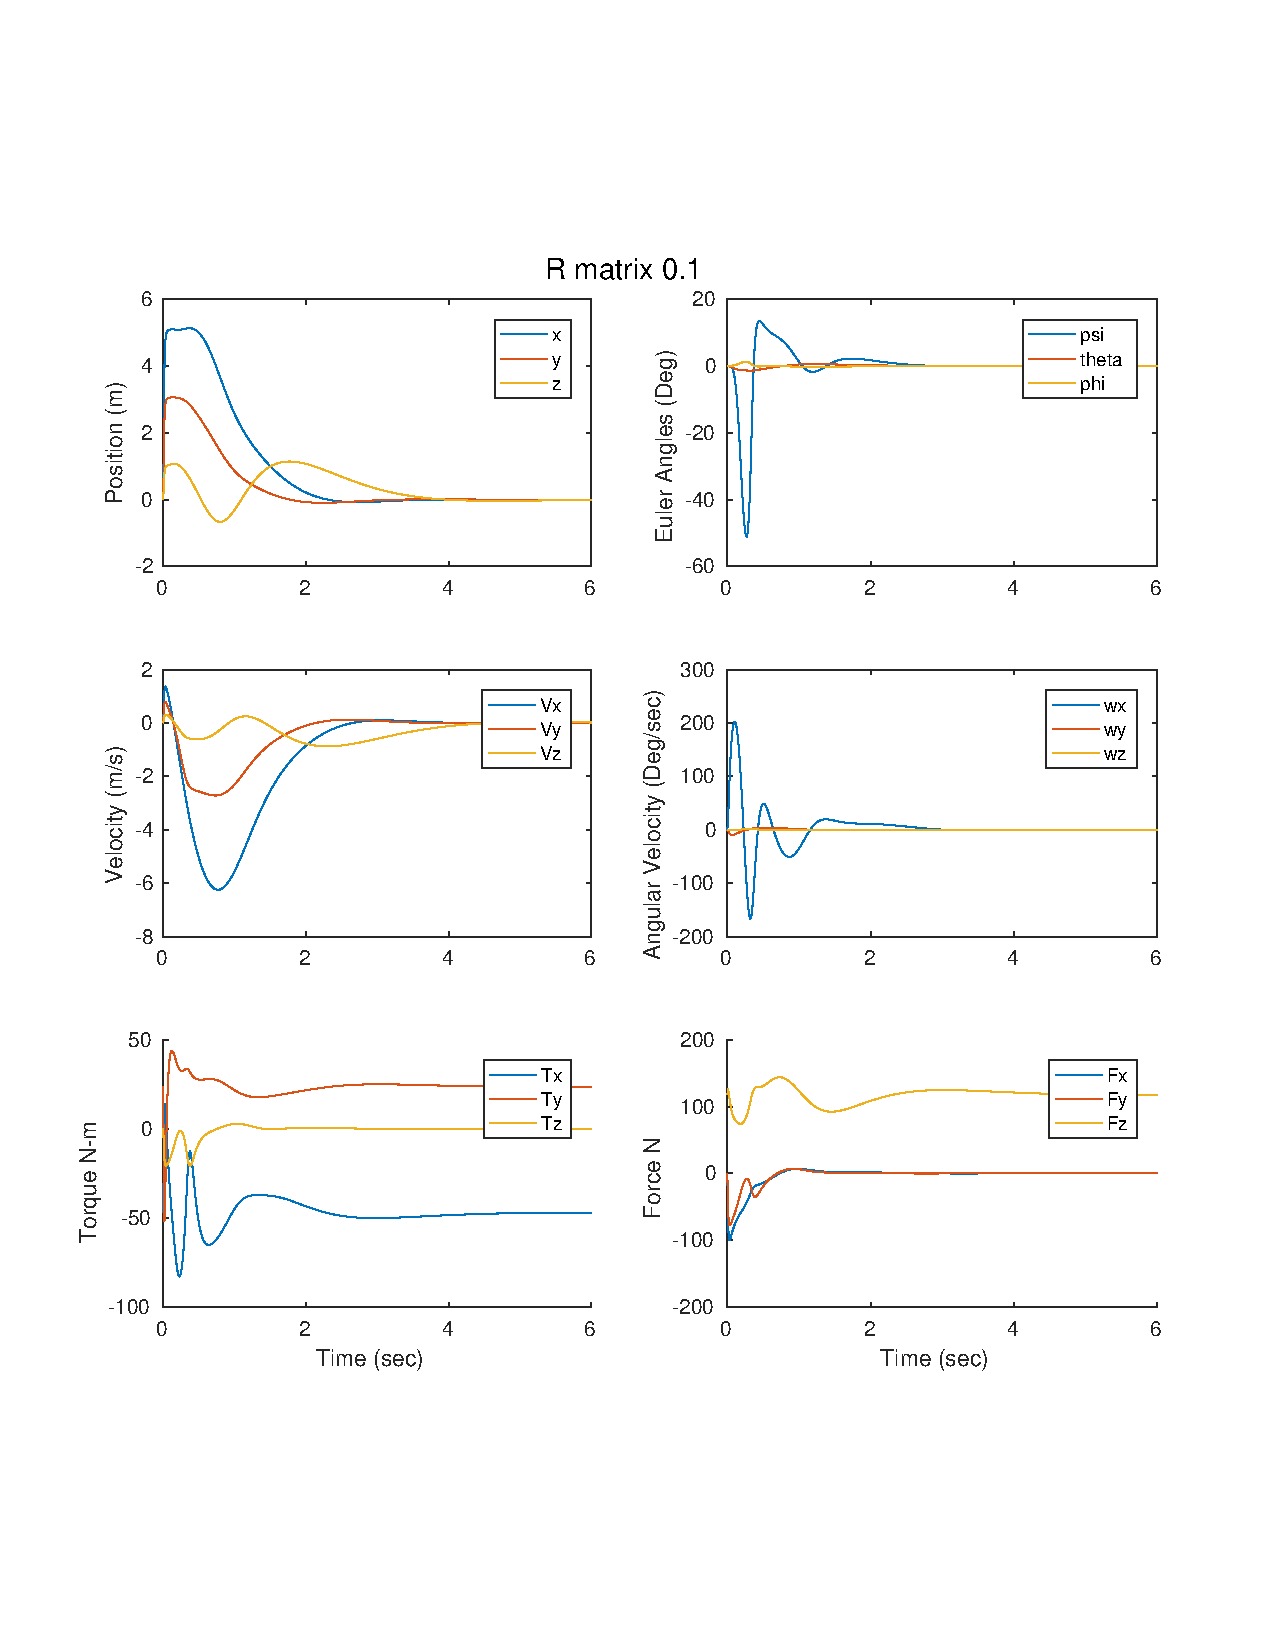
\includegraphics[clip, trim=1cm 4.5cm 1.5cm 4cm, width=0.69\textwidth]{R_0_1_plot_estimated_states.pdf}
    \caption{This figure contains the simulated response with estimated rather than true states.}
    \label{fig:est_states}
\end{figure}

\section{Conclusion}
I learned a ton about the details of implementing an LQR/LQG controller for this project. I spent well over 40 hours getting everything simulated, and really feel like I understand designing an LQR controller with estimated states much better than before the project. 
\end{document}

